\documentclass[a4paper,11pt]{article}

\usepackage[T1]{fontenc}
\usepackage[utf8]{inputenc}
\usepackage{lmodern}
\usepackage[margin=2in]{geometry}
\addtolength{\oddsidemargin}{-.875in}
\addtolength{\evensidemargin}{-.875in}
\addtolength{\textwidth}{1.8in}
\addtolength{\topmargin}{-.875in}
\addtolength{\textheight}{1.75in}
\usepackage{graphicx}
\usepackage{parskip}
\usepackage{cite}
\usepackage{titlesec}

\titlespacing\section{0pt}{12pt plus 4pt minus 2pt}{0pt plus 2pt minus 2pt}
\title{Write-up}
\author{}
\begin{document}
\graphicspath{{images/}}
\section{Introduction}
The Sentences Involving Compositional Knowledge (SICK) dataset consists of 9,840 pairs of sentences. Each sentence pair is labelled as either contradiction, neutral or entailment. The following experiment uses a deep, Siamese, bidirectional, Long Short-Term Memory (LSTM) network to predict sentence entailment using \emph{Word2Vec} embeddings. The data set is split into 4,934 training pairs and 4,906 test pairs.

\section{Word2Vec}
\emph{Word2Vec} is a technology that uses a two-layer neural network to produce a dictionary of vectors from a set of sentences \cite{mikolov2013distributed}. The vector representation of a word is formed using its context and surrounding vocabulary, which enables the embedding process to carry a words semantic meaning. 


It has been demonstrated that words with comparable meanings are embedded as similar vectors, which means they can be manipulated to find synonyms, or to search for similar words in the dictionary of vectors. An example of this being \emph{vec}(king) - \emph{vec}(man) = \emph{vec}(queen).\par  Embedding the entirety of the SICK data set using \emph{Word2Vec} yields a vocabulary of 2,217 individual words.

\section{Network Architecture}
The network reads-in two input sentences as sequences of 300-dimensional \emph{Word2Vec} vectors. 300 dimensions were chosen, as a previous study had success using this embedding dimensionality \cite{mueller2016siamese}. \par Each sentence is fed into a bidirectional LSTM branch. The output from each branch is merged, and input into two dense layers. Softmax is then applied to one-hot encode the output. A diagram of the network architecture is shown in Fig 1.  

\begin{figure}[!htb]
  \begin{center}
    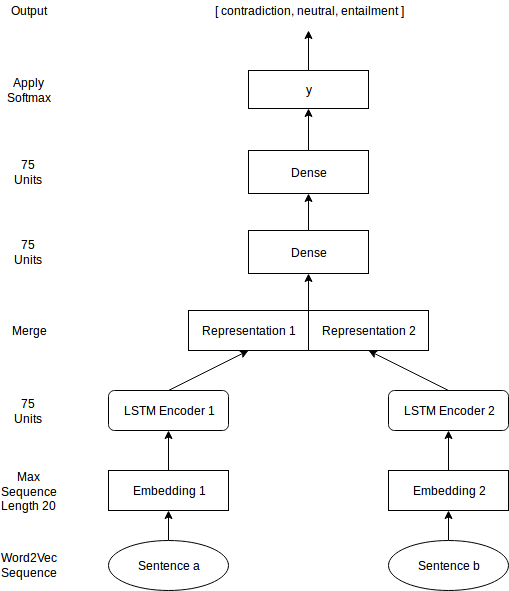
\includegraphics[width=0.7\linewidth]{architecture}
    \caption{Architecture of the network. Two sentences are passed through identical LSTM branches before being processed through two  dense layers and categorised using Softmax.}
    \label{fig:}
  \end{center}
\end{figure}

\section{Results}
An accuracy of 76.03\%, and a loss value of 0.5905 has been achieved when predicting entailment on the unmodified test pairs. Out of 4,906 test predictions, 1,176 were incorrectly classified. \par Accuracy is limited by the number of training examples, which is demonstrated by an accuracy of 77.09\%, and a loss value of 0.5586 when splitting the training/test data sets at 75:25. Out of 2,432 test predictions, 562 were incorrectly classified.  

\section{Further Work}
Accuracy may be improved by generating more training examples. This has been done in another study by replacing random words with synonyms \cite{mueller2016siamese}. \par
The SICK dataset also holds a relatedness score for each sentence pair. Further work could be done to test the network configuration to predict this score by changing the final layer to output a probability. 

\begin{figure}
  \begin{center}
    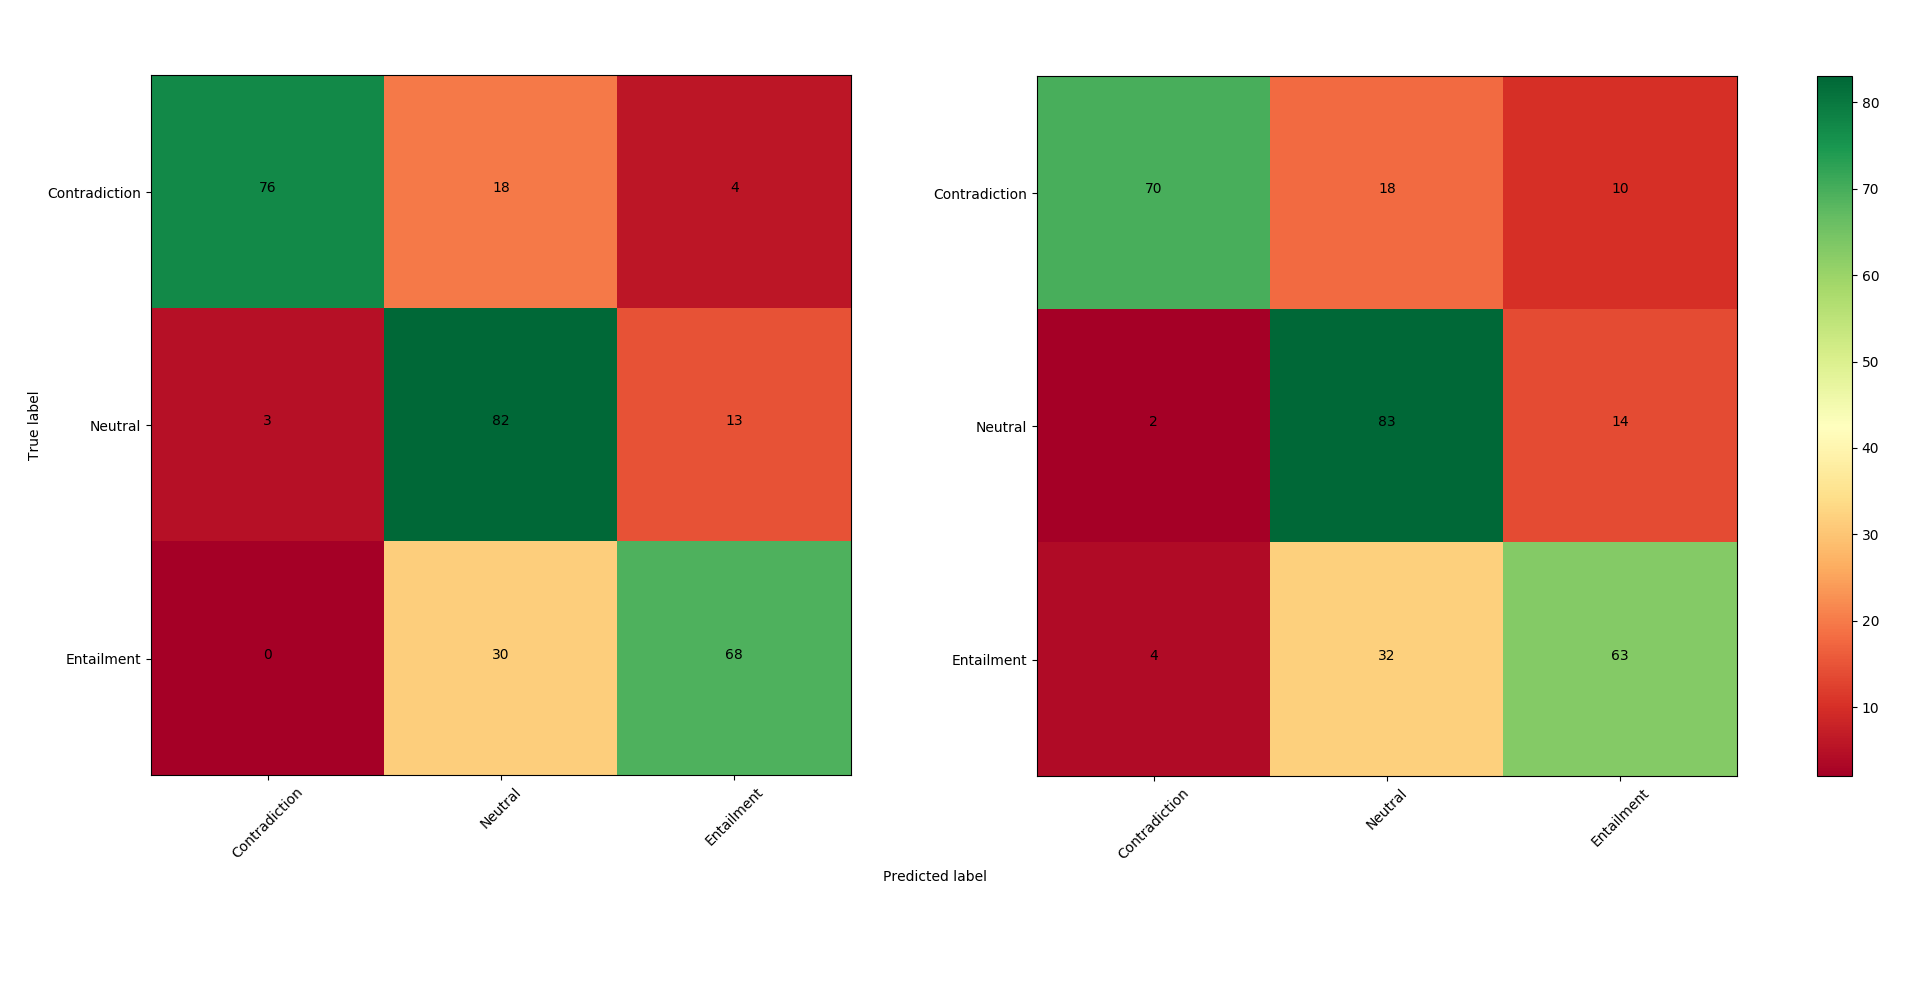
\includegraphics[width=\linewidth]{cm}
    \caption{Normalised confusion matrices showing the number of true labels plotted against their predicted classes. The right-hand side matrix has been trained using a 50:50 train/test split. The left-hand matrix has been trained using a 75:25 train/test split.}
    \label{fig:}
  \end{center}
\end{figure}





\clearpage
\bibliography{citations}{}
\bibliographystyle{plain}
\end{document}
